\chapter{Einführung}
\label{chap:einfuehrung}

\section{Allgemeines zu dieser Vorlage}
\label{sec:Vorlage}
Dieses \LaTeX-Template soll die Erstellung von Berichten erleichtern. Es wurde versucht, in diesem Dokument die wichtigsten Elemente eines Abschlu"sberichtes beispielhaft zu verwenden.
Dazu geh"oren Listen, Tabellen, Bilder, w"ortliche und nicht-w"ortliche Zitate, zitierweisen von Zeitschriftenartikeln, B"uchern, Abschlu"sarbeiten und Webseiten, Gleichungen und Referenzierungen von Kapiteln und Grafiken.

\paragraph{Vollst"andigkeit}
Die Verwendung der Elemente erhebt keinen Anspruch auf Vollst"andigkeit.
Allerdings ist das Internet\cite{onlineLatexHilfe} voll von Hilfen f"ur \LaTeX, deshalb werden Sie keine Probleme haben, wenn Sie z.B. nicht mehr wissen, wie $\gamma$ im Mathematik-Modus geschrieben wird, das herauszufinden.


\section{Meine Arbeit ist zu kurz. Was tun?}
\label{sec:ZuKurz}

Sollten es Schwierigkeiten geben die vorgeschriebene L"ange zu erreichen, vergr"o"sern Sie nicht die Graphiken unangemessen oder schinden ansonsten Seiten, sondern denken "uber folgende Fragen nach:
\begin{enumerate}
\item Habe ich die Literatur zu meinem Thema ausreichend gew"urdigt?
\item Habe ich eine Hinleitung zum Kernthema so geschrieben, dass meine Studienkolleginnen und -kollegen -- ohne Wikipedia zu bem"uhen -- folgen k"onnen?
\item Habe ich die Kernpunkte detailliert genug geschildert?
\item Habe ich alle sinnvollen Experimente tats"achlich durchgef"uhrt, eine Hypothese daran verifiziert oder falsifiziert, das jeweilige Ergebnis nachvollziehbar beschrieben und diskutiert?
\item Habe ich "uber den Tellerrand hinausgesehen und in einem ausf"uhrlichen Ausblick k"unftige sinnvolle Schritte thematisiert?
\end{enumerate}



\chapter{Beispiele}
\label{chap:Beispiele}
In dem Zweiten Kapitel werden einige Beispiele gezeigt, die f"ur die Arbeit relevant sind.


\section{Wie bindet man eine weitere Tex-Datei ein}
\label{sec:tex-dateiEinfuegen}
Es besteht die Möglichkeit einzelne Tex-Dateien manuell einzubinden. Dies hat den Vorteil, dass man die Kapitel logisch trennen kann.\\

Dazu muss man die '00\_settings.tex'-Datei editieren. Im Vorfeld muss im Latex-Verzeichnis eine Datei mit der Endung '.tex' erstellt werden.  Die Dateien werden chronologisch angezeigt.

\FloatBarrier
\begin{figure}[htb]
\begin{lstlisting}[backgroundcolor={\color{white}},
basicstyle={\normalsize\sffamily},
breaklines=true,
frame={bottomline,topline, rightline},
language=HTML,
numbers=left,
showstringspaces=false,
xleftmargin=22pt]	
;
;	% Titelblatt-Datei einbinden. 
;	% Hier muessen der Dateiname und der Pfad stimmen!
;	\include{01_titel}
;           
\end{lstlisting}
  \caption[Beispiel wie eine Tex-Datei eingebunden wird.]{Beschreibt wie man eine weitere Tex-Datei in die '00\_settings.tex'-Datei einbindet.}
\label{lst:Tex-DateienEinbinden}
\end{figure}


\section{Einbinden von Grafiken}
\label{sec:EinbindenVonGrafiken}
Im folgenden wird gezeigt wie man eine Grafik einbindet.

% ### EINBINDEN EINER GRAFIK ###
\FloatBarrier
\begin{figure}[htb]
  \centering  
  
\includegraphics[scale=0.3]{img/kein_bild_vorhanden.eps}
  \caption[Beispiel wie eine Grafik eingebunden wird.]{Beschreibung fuer das Bildverzeichnis am Ende des Dokuments} 
  \label{fig:kein_bild_vorhanden}
\end{figure}

Ein Beispiel wie ein interner Verweis aufgebaut ist (siehe Abbildung \ref{fig:kein_bild_vorhanden}), der die Grafik verlinkt \dots

\section{PDFs einf"ugen}
\label{sec:PDFeinfuegen}
Und so bindet man PDFs ein. Das Keyword 'trim' schneidet den Ausschnitt passend zu. Dabei ist die Reihenfolge der Seiten zu beachten. Zuerst wird links, dann unten, dann rechts und zuletzt die obere Seite angepasst. Zum Schluss muss das Argument 'clip' angef"gut werden, ansonsten schneidet er die PDF nicht zu.

% ### EINBINDEN VON PDFs
\begin{figure}[htb]
  \centering  
  
\includegraphics[width=0.5\textwidth, trim = 10mm 10mm 10mm 10mm, clip]{img/teamfoto.pdf}
  \caption{Das Bild wurde zentriert und wurde wurde mit einer breite von 50 \% der Textweite definiert.} 
  \label{fig:Teambild}
\end{figure}
\FloatBarrier


\section{Figur genau hier einf"ugen}
\label{sec:FigurHierEinfuegen}
Um eine Figur an einer bestimmten stelle einzubinden muss man den Paramter [H] verwenden.

\FloatBarrier
\begin{figure}[htb]
\begin{lstlisting}[backgroundcolor={\color{white}},
basicstyle={\normalsize\sffamily},
breaklines=true,
frame={bottomline,topline, rightline},
language=HTML,
numbers=left,
showstringspaces=false,
xleftmargin=22pt]	
; 
;	\begin{figure}[htb]
;	...
;	\end{figure}
;
\end{lstlisting}
  \caption[Die Anweisung, wie man eine Figure genau hier einbindet.]{Das Beispiel veranschaulicht, wie man eine Figur genau an einer bestimmten Stelle einbindet.}
\label{lst:FigurGenauHier}
\end{figure}


\section{Tabellen}
\label{sec:Tabellen}
Tabellen sind in Latex nicht ganz einfach zu verwalten. Man sollte sich vor dem Eingeben einer Tabelle genaue Gedanken machen, wie sie aussehen soll und welche Inhalte wo hingehören. Spalten im Nachhinein zu vertauschen, bedeutet einen vergleichsweise großen Aufwand.

\subsection{Tabelle 1}
\label{subsection:Tabelle1}

% ### HIER KOMMT EINE TABELLE ###
\newcolumntype{b}{X}
\newcolumntype{s}{>{\hsize=.2\hsize}X}
\begin{table}[H]
\begin{tabularx}{\textwidth}{sb}
%{X|X}
\textbf{Spalte1} & \textbf{Spalte2}\\
\hline

Zelle11 & Zelle12.  \\ \hline

Zelle21 & Zelle22. \\ \hline

\end{tabularx}
\caption[Eine Einfache Tabelle zum darstellen von Werten]{Das ist eine einfache Tabelle, die  zwei Spalten und 3 Zeilen hat.
\label{tab:Tabelle1}}
\end{table}
\FloatBarrier

\subsection{Tabelle 2}
\label{subsection:Tabelle2}

\begin{table}[H]\vspace{1ex}\centering
\begin{tabular*}{12cm}{ll|@{\extracolsep\fill}cccc}
&&\multicolumn{4}{c}{Verfahren} \\
&& A  & B &  C & D\\\hline
\multirow{5}*{\rotatebox{90}{Datens"atze}}
& Proband 1 &  negativ  & negativ & negativ & negativ  \\%\cline{2-6}
& Proband 2 &  negativ  & negativ & negativ & negativ  \\%\cline{2-6}
& Proband 3 &  negativ  & negativ & negativ & negativ  \\%\cline{2-6}
& Proband 4 &  negativ  & negativ & \textbf{positiv} & bla \\%\cline{2-6}
& Proband 5 &  negativ  & negativ & negativ & negativ  \\\hline
\end{tabular*}
\caption[Beispieltabelle]{Das ist ein Beispiel f"ur eine recht komplexe Tabelle.
Nicht der gesamte Text der Tabellenunterschrift sollte im Tabellenverzeichnis auftauchen.
Hier wurde der beste Wert \textbf{fett} markiert.
\label{tab:Tabelle2}}
\vspace{2ex}\end{table}




\section{Aufz"ahlungen}
\label{sec:Aufzaehlungen}

\subsection{Punkt}
\label{subsec:Punkt}

% ### VERSCHACHTELTE AUFZAEHLUNGEN ###
\begin{itemize}
\item Die Darstellung der Dokumentation in verschiedenen gängigen Browsern in aktueller Version: \textit{Internet Explorer}, \textit{Edge}, \textit{Google Chrome} und \textit{Mozilla Firefox}.
\item Die Korrektheit der Flussdiagramme und der Proportionen von Knoten und Kanten.
\item Die korrekte Funktion der JQuery-Funktionen (Erfordert teilweise das Zulassen von Skripts im Browser)
\begin{itemize}
\item Ein- und Ausklappen von Labels durch Betätigen der Buttons.
\item Wechseln zwischen Reitern im Topmenü und Hervorheben des aktuellen Reiters.
\item Wechseln zwischen Dateien in Marginalmenü und Hervorheben der aktuellen Datei.
\item Betätigen der Links zu Makros und Labels, die an anderer Stelle im Projekt definiert sind.
\item Öffnen der Ablaufgraphen in der Vollbildansicht in einem neuen Browser-Tab.
\item Anwenden einer speziellen Formatierung und Verbergen der Menüs im Druck-Layout beim Betätigen des Druck-Buttons.
\end{itemize}
\end{itemize}

\subsection{Zahlen}
\label{subsec:Zahlen}

\begin{enumerate}
\item Es gibt verschiedene Arten Listen aufzulisten
\item In diesem Dokument wurden drei Arten von Auflistungen vorgestellt. 
\end{enumerate}


\section{Fu{\ss}zeile}
\label{sec:Fusszeile}


Eine Quelle in der Fußzeile lässt sich \textit{folgendermaßen}\footnote{\url{http://my/url.com}, (Zugriff am 17.10.2017)} realisieren.


\section{Listing}
\label{sec:Listing}

\paragraph{Code}
Source Code kann durchaus sparsam dosiert in der Arbeit auftauchen.
Aber nicht vollst"andig und als Anhang (siehe Anhang \ref{cap:Anhang}), sondern in sinnvollen Ausschnitten, wenn anhand des Code-Fragments ein Sachverhalt erl"autert werden soll.

\subsection{Listing 1}
\label{subsec:Listing1}

\FloatBarrier
\begin{figure}[htb]
\begin{lstlisting}[language=C++, breaklines=true, basicstyle=\small, numbers=none]
// Das ist ein Beispiel fuer ein Codefragment
int a = 7;
int b = 3;
int c = 10;
a *= 2;
c -= b + a++;
std::cout << "c = " << c << std::endl;
\end{lstlisting}
  \caption[Beispiel eines einfachesn Codefragments.]{Ein einfache Codefragment, dass eine mathematische Berechnung durchf"uhrt.}
\label{lst:Codefragment}
\end{figure}


\subsection{Listing 2}
\label{subsec:Listing 2}

Das hier ist ein Listing, das ASCII-Code einbettet

% ### Das hier ist ein Listing, das ASCII-Code einbettet ###
\FloatBarrier
\begin{figure}[htb]
\begin{lstlisting}[backgroundcolor={\color{white}},
basicstyle={\normalsize\sffamily},
breaklines=true,
frame={bottomline,topline, rightline},
language=HTML,
numbers=left,
showstringspaces=false,
xleftmargin=22pt]	
; This is the description of a test case.
;
;           .------------------------------.
;           |          Start [0]           |
;           '------------------------------'
;                           |
;                           v
;       .---------------------------------------.
;       |             Some content		        |
;       '---------------------------------------'
;                           |
;                           v
;           .------------------------------.
;           |          Return [1]          |
;           '------------------------------'
\end{lstlisting}
  \caption[Ein Listing, welches zusätzliche die Zeilen anzeigt.]{Kann verwendet werden, um ein einfach Diagramm selber zu erstellen oder Code einzubinden.}
\label{lst:Diagramm}
\end{figure}

\section{Formeln}
\label{sec:Formeln}

Formeln werden nach folgendem Schema angegeben

\begin{equation}
g = n\cdot l_n + l_i + l_l + 1.
\label{gle:Laenge}
\end{equation}


\section{Zitierung}\label{zitierung}

Es ist verpflichtend, alle Quellen und Hilfmittel anzugeben, die verwendet werden.
Dabei ist die w"ortliche Zitierung in der Informatik selten, schon deshalb, weil viele Quellen englischsprachig sind und ein englisches w"ortliches Zitat in einer deutschen Arbeit keinen Sinn macht.
Meist werden Gedanken, Ideen und Methoden aus Quellen entnommen.
Das Zitat kommt dann an den Schlu"s des letzten Satzes des Abschnittes, der z.B. die Methode beschreibt \cite{wissentschaftlichesArbeitMitLatex}.
Bitte beachten Sie, dass das Zitat \textbf{vor} dem abschli"senden Punkt erscheint und nicht danach!

Alternativ wird zu Beginn oder am Ende der Beschreibung der Methode die Quelle mit Hilfe einer Phrase wie:
\begin{quote}
Angreifer, die Zugang zum PC haben m"ochten nutzen die Anwendungen von dem Benutzer, die selten bis garnicht verwendet werden. Sobald der Benutzer diese Hintert"uren geschlossen hat kann man sich mit den seinen eigenen Daten sicherer f"uhlen \cite{ctWindowsEinfachAbsichern}.
\end{quote}


Als ein hilfreiches Werkzeug zum Auffinden von wissenschaftlichen Artikeln hat sich \url{http:\\\\scholar.google.com} erwiesen.

\paragraph{Zitierung von Internetseiten}
Grunds"atzlich ist das Zitieren von Internetseiten so weit wie m"oglich zu vermeiden.
Internetseiten k"onnen pl"otzlich offline sein, der Inhalt kann sich "andern, manchmal ist der Autor unklar.
Genau das Gegenteil erwartet man von einer \emph{zitierf"ahigen} Quelle.
Dennoch l"a"st sich der Hinweis auf eine Internetseite manchmal nicht vermeiden.
In diesen F"allen versuchen Sie, den Autor herauszufinden und in die Quellenangabe einzuf"ugen.
Wichtig ist der Hinweis auf das letzte Zugriffdatum \cite{zitieren13}.
Au"serdem wird meistens erwartet die Seiten lokal zu speichern und ebenso in elektronischer Form zu der Arbeit hinzuzuf"ugen.

Besonders Wikipedia-Seiten sind kritisch zu bewerten. In Wikipedia selbst ist zu lesen:
\begin{quote}
\glqq In wissenschaftlichen Arbeiten sollte auf das Zitieren von Wikipedia-Artikeln nach M"oglichkeit verzichtet werden, da keine Garantie f"ur den Inhalt gegeben werden kann.
Zudem folgt Wikipedia derzeit nur sehr rudiment"ar den Ma"sgaben des wissenschaftlichen Arbeitens und die Artikelqualit"at variiert stark, weswegen es als wissenschaftliche Quelle oft ausscheidet.\grqq \cite{zitieren13a}
\end{quote}
Dem ist nichts hinzuzuf"ugen.

\section{Literatur}
\label{sec:Literatur}

Wie bereits in der ReadMe.txt angedeutet wird biblatex f"ur das Literaturverzeichnis verwendet. Es k"onnen drei verschiedene Arten von Literatur angegeben werden:

\begin{itemize}
\item B"ucher\cite{wissentschaftlichesArbeitMitLatex}
\item Internetquellen\cite{zitieren13a}
\item Zeitschriftenartikel
\end{itemize}

Die Literatur wird selbst in einer seperaten Datei (Literatur.bib) eingetragen und erh"alt einen eindeutigen Namen. Mit dem eindeutigen Namen kann man in der Arbeit jeder Literatur "uberall einfuegen. 


\FloatBarrier
\begin{figure}[htb]
\begin{lstlisting}[backgroundcolor={\color{white}},
basicstyle={\normalsize\sffamily},
breaklines=true,
frame={bottomline,topline, rightline},
language=HTML,
numbers=left,
showstringspaces=false,
xleftmargin=22pt]	
;
;	\cite{wissentschaftlichesArbeitMitLatex}
;           
\end{lstlisting}
  \caption[Beschreibt wie man eine Literaturenquelle einbindet.]{Zeigt auf wie eine Quellenangabe in Latex eingef"ugt werden muss.}
\label{lst:literaturenquelle}
\end{figure}


\begin{landscape}


\section{Einzelne Seite im Querformat}
\label{sec:Querformat}


Es besteht die M"oglichkeit einzelne Seite queer darzustellen. M"ochte man beispielsweise ein UML-Diagramm komplett vorstellen kann es durchaus sinn machen.

\section{Latex cheat sheet und PDFs einbinden}
\label{sec:cheatsheet}

Im Folgenden wird gezeigt wie man eine PDF-Datei einbindet. In der PDF Datei sind n"utzliche Anweisungen von Latex enthalten, welche hier nicht n"aher betrachtet wurden.

\end{landscape}

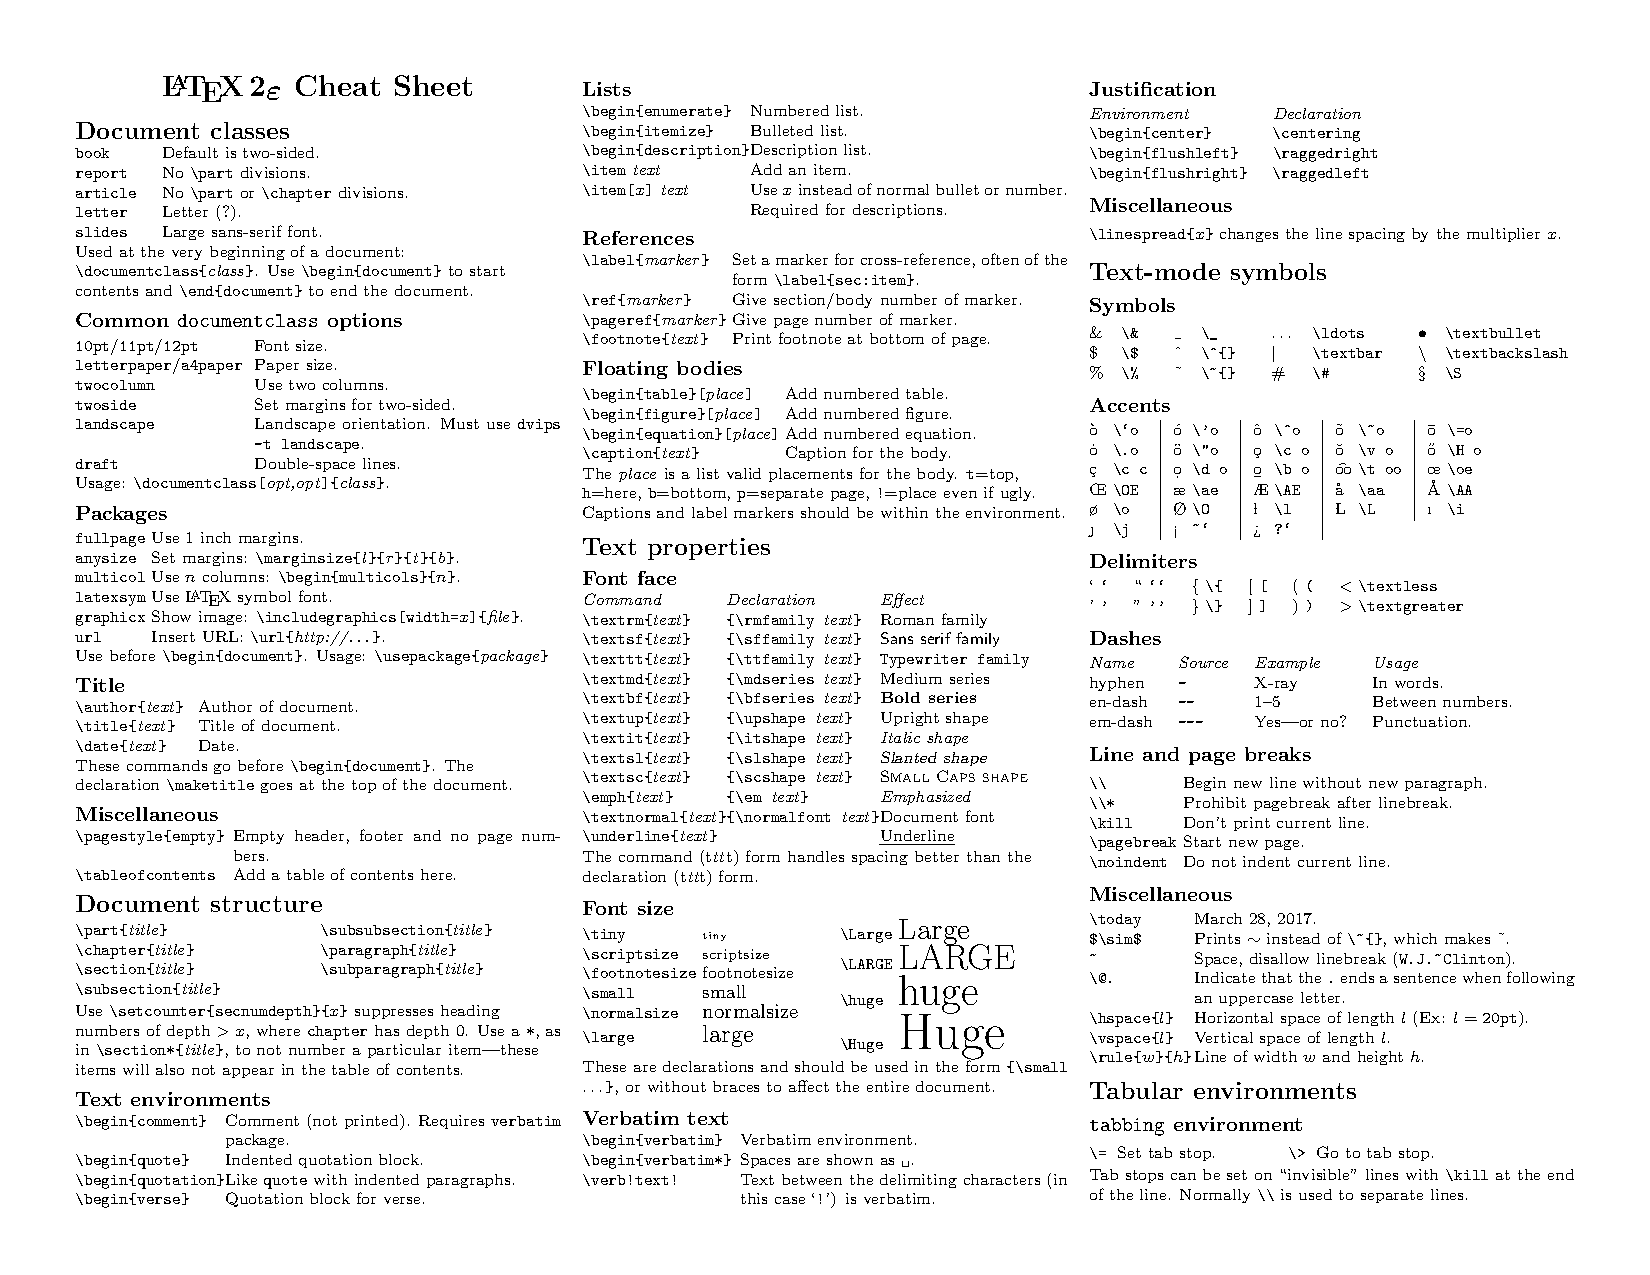
\includepdf[landscape=true,pages=-]{img/latexsheet.pdf} 



\cleardoublepage
